% ==============================================================================
% Modelo para Monografia de Projeto de Graduação - Ciência da Computação (em Português)
% Prof. Vítor E. Silva Souza - NEMO/UFES :: DI/UFES :: PPGI/UFES
% Com adaptações feitas pelo Colegiado de Engenharia de Computação / CT / UFES e pela profª. Monalessa Perini Barcellos (NEMO/UFES).
%
%
% Baseado em abtex2-modelo-trabalho-academico.tex, v-1.9.2 laurocesar
% Copyright 2012-2014 by abnTeX2 group at http://abntex2.googlecode.com/ 
%
% This work may be distributed and/or modified under the conditions of the LaTeX 
% Project Public License, either version 1.3 of this license or (at your option) 
% any later version. The latest version of this license is in
% http://www.latex-project.org/lppl.txt.
%
% IMPORTANTE:
% Instruções encontram-se espalhadas pelo documento. Para facilitar sua leitura,
% tais instruções são precedidas por (*) -- utilize a função localizar do seu
% editor para passar por todas elas.
% ==============================================================================

% Usa o estilo abntex2, configurando detalhes de formatação e hifenização.
\documentclass[
	12pt,				% Tamanho da fonte.
	openright,			% Capítulos começam em página ímpar (insere página vazia caso preciso).
	oneside,			% Para impressão em verso e anverso. Oposto a oneside.
	a4paper,			% Tamanho do papel.
	english,			% Idioma adicional para hifenização.
	french,				% Idioma adicional para hifenização.
	spanish,			% Idioma adicional para hifenização.
	brazil				% O último idioma é o principal do documento.
	]{abntex2}



%%% Importação de pacotes. %%%

% Conserta o erro "No room for a new \count". 
% O comando \reserveinserts deve ser comentado ou não, dependendo da versão do LaTeX.
\usepackage{etex}
%\reserveinserts{28}

% Usa a fonte Latin Modern.
\usepackage{lmodern}

% Seleção de códigos de fonte.
\usepackage[T1]{fontenc}

% Codificação do documento em Unicode.
\usepackage[utf8]{inputenc}

% Usado pela ficha catalográfica.
\usepackage{lastpage}

% Indenta o primeiro parágrafo de cada seção.
\usepackage{indentfirst}

% Controle das cores.
\usepackage[usenames,dvipsnames]{xcolor}

% Inclusão de gráficos.
\usepackage{graphicx}

% Tabularx package: melhor controle de leiaute de tabelas.
\usepackage{tabularx}

% Inclusão de páginas em PDF diretamente no documento (para uso nos apêndices).
\usepackage{pdfpages}

% Para melhorias de justificação.
\usepackage{microtype}

% Citações padrão ABNT.
\usepackage[brazilian,hyperpageref]{backref}
\usepackage[alf]{abntex2cite}	
\renewcommand{\backrefpagesname}{Citado na(s) página(s):~}		% Usado sem a opção hyperpageref de backref.
\renewcommand{\backref}{}										% Texto padrão antes do número das páginas.
\renewcommand*{\backrefalt}[4]{									% Define os textos da citação.
	\ifcase #1
		Nenhuma citação no texto.
	\or
		Citado na página #2.
	\else
		Citado #1 vezes nas páginas #2.
	\fi}

% \rm is deprecated and should not be used in a LaTeX2e document
% http://tex.stackexchange.com/questions/151897/always-textrm-never-rm-a-counterexample
\renewcommand{\rm}{\textrm}

% Inclusão de símbolos não padrão.
\usepackage{amssymb}
\usepackage{eurosym}

% Para utilizar \eqref para referenciar equações.
\usepackage{amsmath}

% Permite mostrar figuras muito largas em modo paisagem com \begin{sidewaysfigure} ao invés de \begin{figure}.
\usepackage{rotating}

% Permite customizar listas enumeradas/com marcadores.
\usepackage{enumitem}

% Permite inserir hiperlinks com \url{}.
\usepackage{bigfoot}
\usepackage{hyperref}

% Permite usar o comando \hl{} para evidenciar texto com fundo amarelo. Útil para chamar atenção a itens a fazer.
\usepackage{soulutf8}

% Colorinlistoftodos package: to insert colored comments so authors can collaborate on the content.
\usepackage[colorinlistoftodos, textwidth=20mm, textsize=footnotesize]{todonotes}
\newcommand{\aluno}[1]{\todo[author=\textbf{Aluno},color=green!30,caption={},inline]{#1}}
\newcommand{\professor}[1]{\todo[author=\textbf{Professor},color=red!30,caption={},inline]{#1}}

% Permite inserir espaço em branco condicional (incluído no texto final só se necessário) em macros.
\usepackage{xspace}

% Permite incluir listagens de código com o comando \lstinputlisting{}.
\usepackage{listings}
\usepackage{caption}
\DeclareCaptionFont{white}{\color{white}}
\DeclareCaptionFormat{listing}{\colorbox{gray}{\parbox{\textwidth}{#1#2#3}}}
\captionsetup[lstlisting]{format=listing,labelfont=white,textfont=white}
\renewcommand{\lstlistingname}{Listagem}
\definecolor{mygray}{rgb}{0.5,0.5,0.5}
\lstset{
	basicstyle=\scriptsize,
	breaklines=true,
	numbers=left,
	numbersep=5pt,
	numberstyle=\tiny\color{mygray}, 
	rulecolor=\color{black},
	showstringspaces=false,
	tabsize=2,
    inputencoding=utf8,
    extendedchars=true,
    literate=%
    {é}{{\'{e}}}1
    {è}{{\`{e}}}1
    {ê}{{\^{e}}}1
    {ë}{{\¨{e}}}1
    {É}{{\'{E}}}1
    {Ê}{{\^{E}}}1
    {û}{{\^{u}}}1
    {ù}{{\`{u}}}1
    {â}{{\^{a}}}1
    {à}{{\`{a}}}1
    {á}{{\'{a}}}1
    {ã}{{\~{a}}}1
    {Á}{{\'{A}}}1
    {Â}{{\^{A}}}1
    {Ã}{{\~{A}}}1
    {ç}{{\c{c}}}1
    {Ç}{{\c{C}}}1
    {õ}{{\~{o}}}1
    {ó}{{\'{o}}}1
    {ô}{{\^{o}}}1
    {Õ}{{\~{O}}}1
    {Ó}{{\'{O}}}1
    {Ô}{{\^{O}}}1
    {î}{{\^{i}}}1
    {Î}{{\^{I}}}1
    {í}{{\'{i}}}1
    {Í}{{\~{Í}}}1
}



%%% Definição de variáveis. %%%

% (*) Substituir os textos abaixo com as informações apropriadas.
\titulo{O mundo de Super Mario Odyssey}
\autor{João Victor Ricardo de Andrade}
\local{São Mateus, ES}
\data{\the\year}
\orientador {Leonardo José Silvestre}
\instituicao{
  Universidade Federal do Espírito Santo -- UFES
  \par
  Departamento de Computação e Eletrônica (DCEL)}
\tipotrabalho{Monografia (PG)}

% Macros específicas do trabalho.
% (*) Inclua aqui termos que são utilizados muitas vezes e que demandam formatação especial.
% Os exemplos abaixo incluem i* (substituindo o asterisco por uma estrela) e Java com TM em superscript.
% Use sempre \xspace para que o LaTeX inclua espaço em branco após a macro somente quando necessário.
\newcommand{\istar}{\textit{i}$^\star$\xspace}
\newcommand{\java}{Java\texttrademark\xspace}
\newcommand{\latex}{\LaTeX\xspace}



%%% Configurações finais de aparência. %%%

% Altera o aspecto da cor azul.
\definecolor{blue}{RGB}{41,5,195}

% Informações do PDF.
\makeatletter
\hypersetup{
	pdftitle={\@title}, 
	pdfauthor={\@author},
	pdfsubject={\imprimirpreambulo},
	pdfcreator={LaTeX with abnTeX2},
	pdfkeywords={abnt}{latex}{abntex}{abntex2}{trabalho acadêmico}, 
	colorlinks=true,				% Colore os links (ao invés de usar caixas).
	linkcolor=blue,					% Cor dos links.
	citecolor=blue,					% Cor dos links na bibliografia.
	filecolor=magenta,				% Cor dos links de arquivo.
	urlcolor=blue,					% Cor das URLs.
	bookmarksdepth=4
}
\makeatother

% Espaçamentos entre linhas e parágrafos.
\setlength{\parindent}{1.3cm}
\setlength{\parskip}{0.2cm}



%%% Páginas iniciais do documento: capa, folha de rosto, ficha, resumo, tabelas, etc. %%%

% Compila o índice.
\makeindex

% Inicia o documento.
\begin{document}

% Brasão da instituição.
\begin{figure}
	\centering
	
\includegraphics[width=.20\textwidth]{figuras/brasao.jpg} 
	\label{fig-brasao}
\end{figure}

\begin{center}
	\textbf{\textsf{UNIVERSIDADE FEDERAL DO ESPÍRITO SANTO}}
	
	\textbf{\textsf{DEPARTAMENTO DE COMPUTAÇÃO E ELETRÔNICA}}
	
	\large{\textbf{\textsf{  }}}
	
	\large{\textbf{\textsf{  }}}
\end{center}

% Retira espaço extra obsoleto entre as frases.
\frenchspacing

% Capa do trabalho.
\imprimircapa

% Folha de rosto (o * indica que haverá a ficha bibliográfica).
\imprimirfolhaderosto*


% Insere o sumário.
\pdfbookmark[0]{\contentsname}{toc}
\tableofcontents*
\cleardoublepage


%%% Início da parte de conteúdo do documento. %%%

% Marca o início dos elementos textuais.
\textual

% Inclusão dos capítulos.
% (*) Para facilitar a organização, os capítulos foram divididos em arquivo separados e colocados dentro da.
% pasta capitulos/. Caso o aluno prefira trabalhar com um só arquivo, basta substituir os comandos \include 
% pelos conteúdos dos arquivos que estão sendo incluídos, excluindo a pasta capitulos/ em seguida.
% ==============================================================================
% PG - Nome do Aluno
% Capítulo 1 - Introdução
% ==============================================================================
\chapter{Descrição}
\label{sec-desc}

\par Mario Odyssey foi a 7ª aventura (e última até o momento) de Mario, sendo lançado em 2017. Mario Odyssey segue o mesmo esquema de história de títulos anteriores e presta certa homenagem a eles, em especial ao Mario 64, tendo um reino inteiro dedicado ao título do Nintendo 64 que deu modelo aos jogos de plataforma 3D. Assim como todos os jogos do Mario, Odyssey começa com a princesa Peach sendo raptada mais uma vez por Bowser, que derrota Mario e o derruba de sua aeronave. Após isso, ele acorda em um reino desconhecido (Cap Kingdom) e se encontra com Cappy (personagem que vai ser seu parceiro durante toda a sua jornada), que teve sua irmã Tiara raptada por Bowser.
\par Unidos pelo objetivo de derrotar Bowser e resgatar seus amigos, Cap e Mario derrotam um dos capangas de Bowser e vão até a nave Odyssey, restaurando-a com a ajuda das Power Moons, o que acontecerá com frequência durante sua passagem pelos reinos. São 14 reinos que Mario e Cappy percorrem durante sua aventura, sendo eles: Cap Kingdom, Cascade Kingdom, Sand Kingdom, Wooded Kingdom, Lake Kingdom, Cloud Kingdom, Lost Kingdom, Metro Kingdom, Seaside Kingdom, Snow Kingdom, Luncheon Kingdom, Ruined Kingdom, Bowser's Kingdom, Moon Kingdom. Além desses, temos mais 3 reinos adicionais que são jogáveis após o encerramento da história: Mushroom Kingdom, Dark Side e Darker Side. Na maioria dos reinos, Mario os visita com o objetivo de perseguir Bowser, enquanto Bowser visita os reinos para roubar algo para seu casamento (e.g. no Cap Kingdom ele rouba Tiara, e no Wooded Kingdom ele rouba as flores para seu casamento). 
\par Uma das principais novidades de Odyssey foi o sistema de capturas que ocorrem quando Mario joga Cappy na cabeça de boa parte dos personagens, passando a ‘possuir’ aquele personagem e adquirindo as habilidades do mesmo, que o ajudam a pular obstáculos que são impossíveis para Mario, voar pelo cenário, atirar projéteis e etc. variando de acordo com o tipo de captura realizada.
O presente trabalho tem por objetivo principal modelar, por meio de um programa escrito em Prolog, alguns aspectos do mundo de Mario Odyssey, apresentando seus reinos, alguns fatos da história e personagens.

\chapter{Diagrama Ontológico}
\label{sec-diag-ontol}

\rotatebox{90}{
	\begin{minipage}{0.75\textheight}
		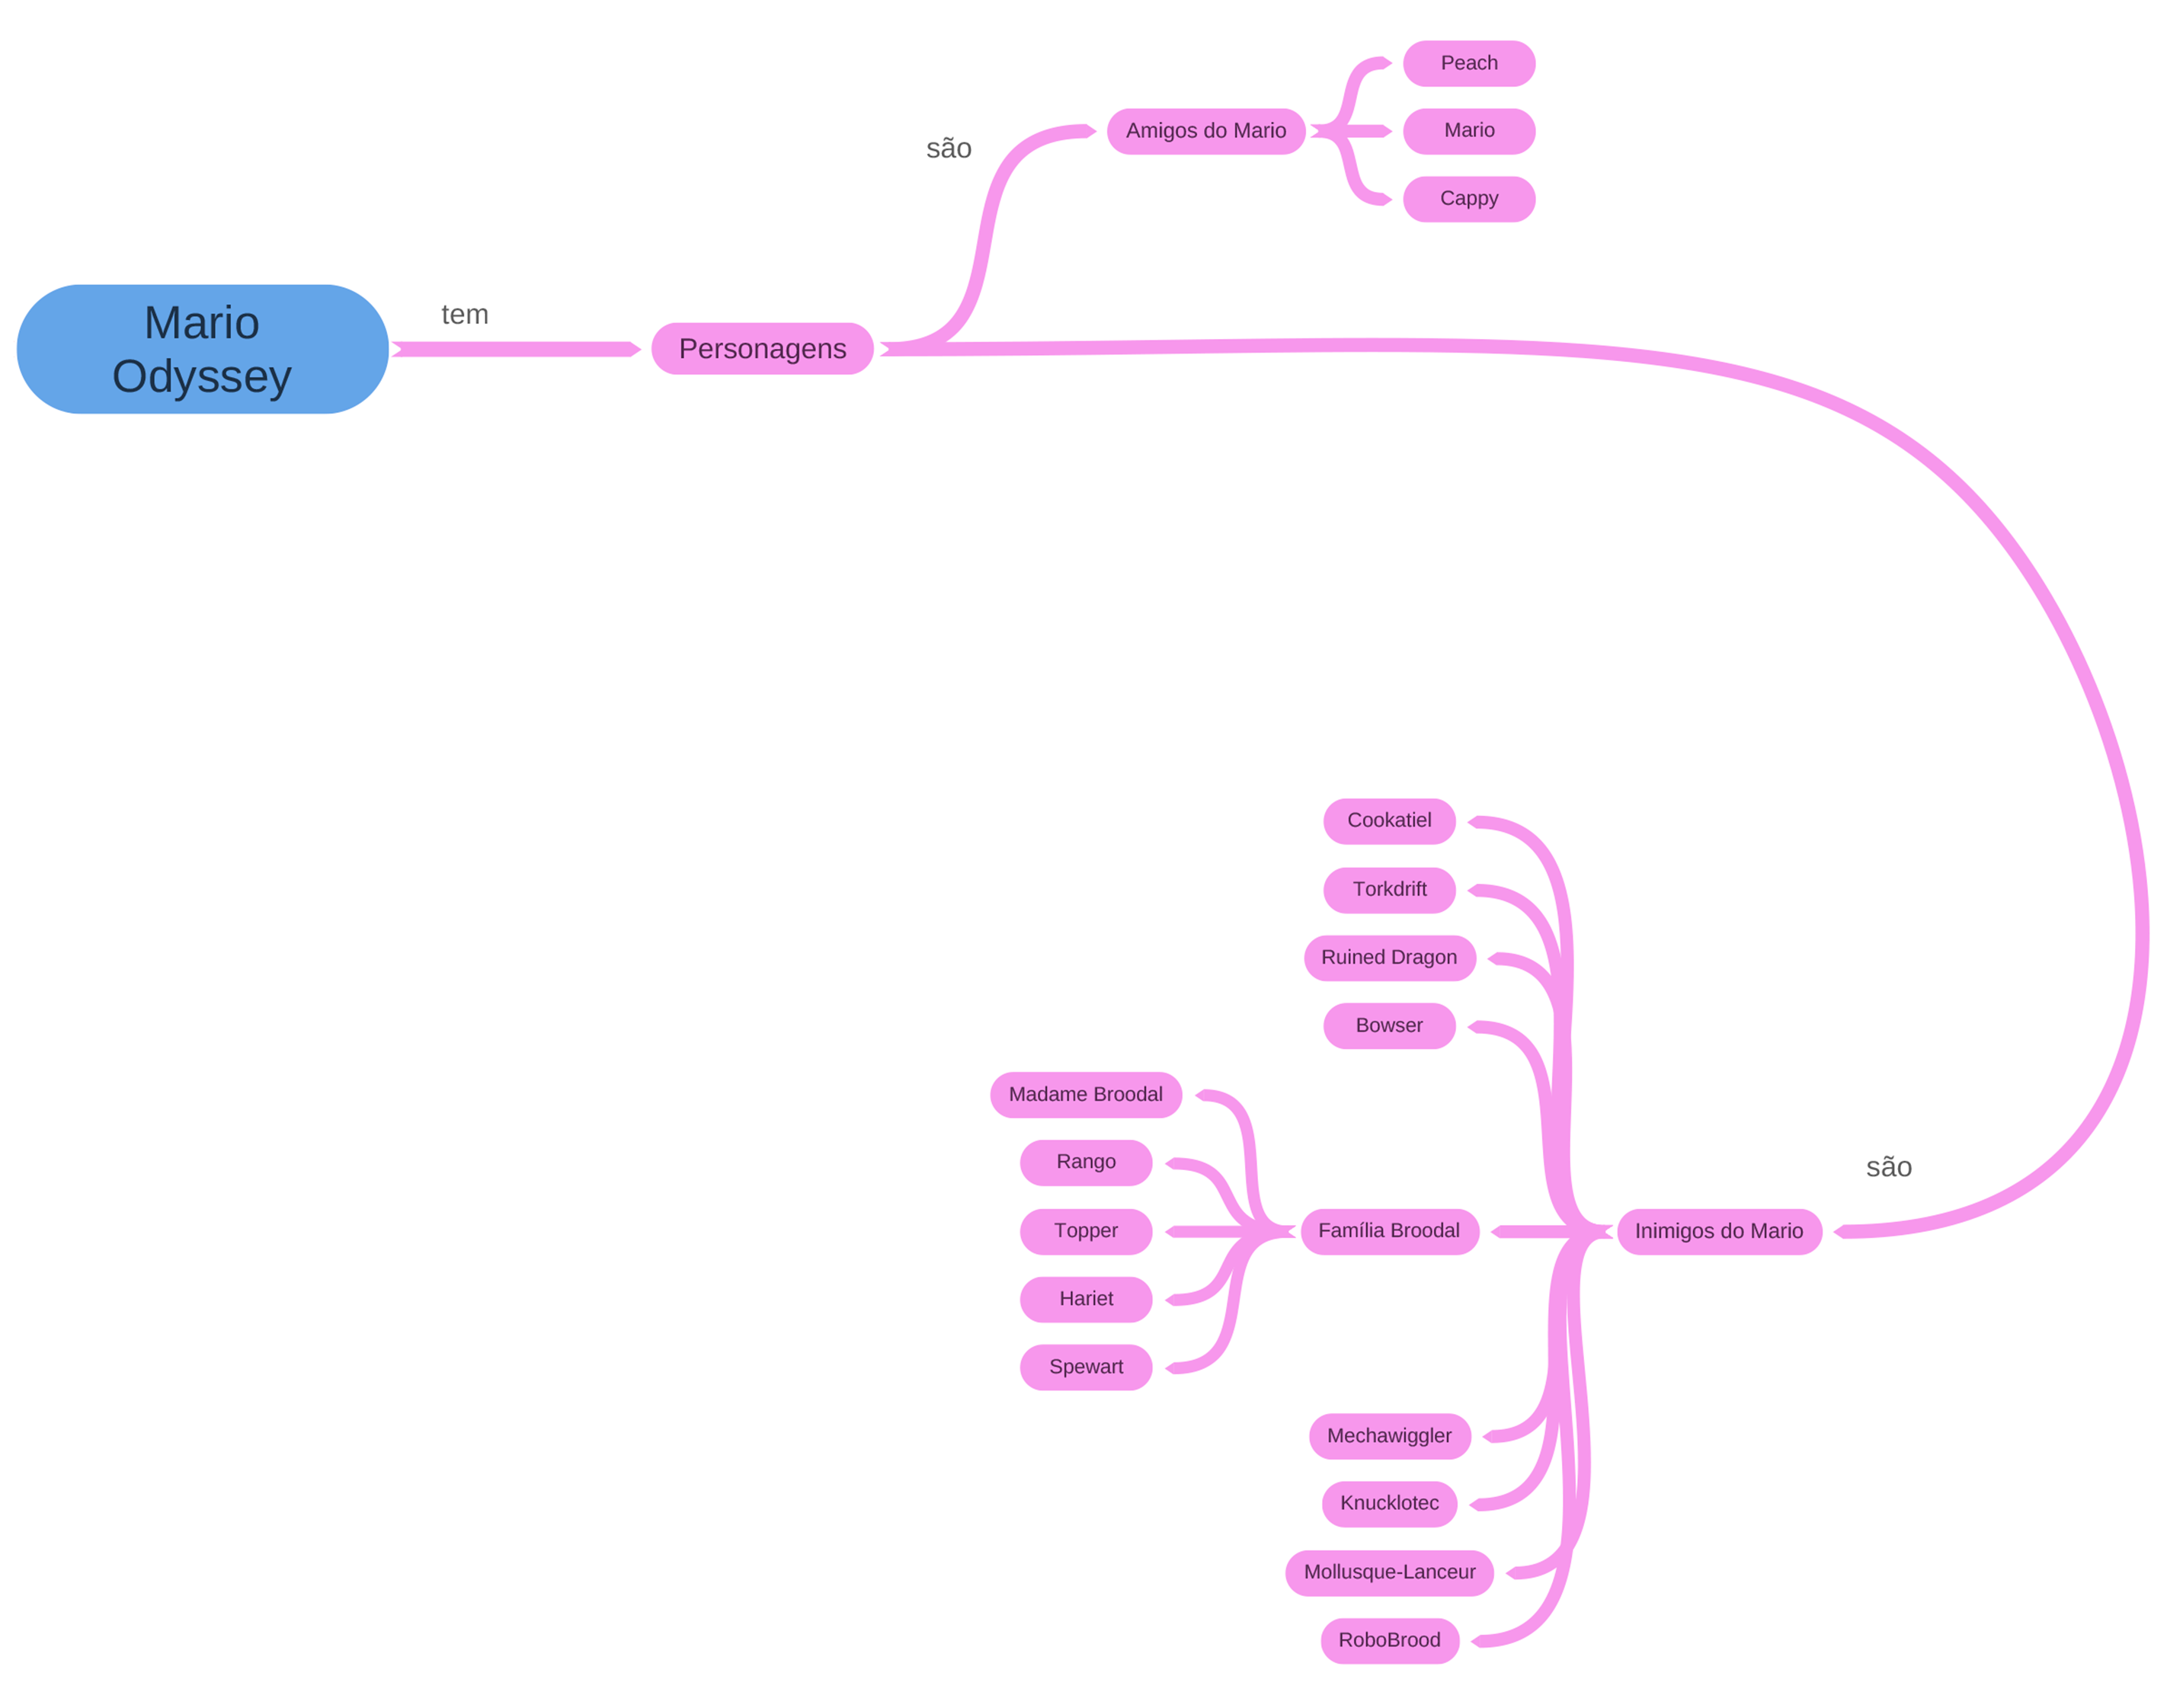
\includegraphics[width=\textwidth]{figuras/fig-diag-1} 
	    \captionof{figure}{Primeira parte do diagrama ontológico.}
   		\label{fig-intro-diag1}	
	\end{minipage}
	}

\begin{sidewaysfigure}
	\centering
	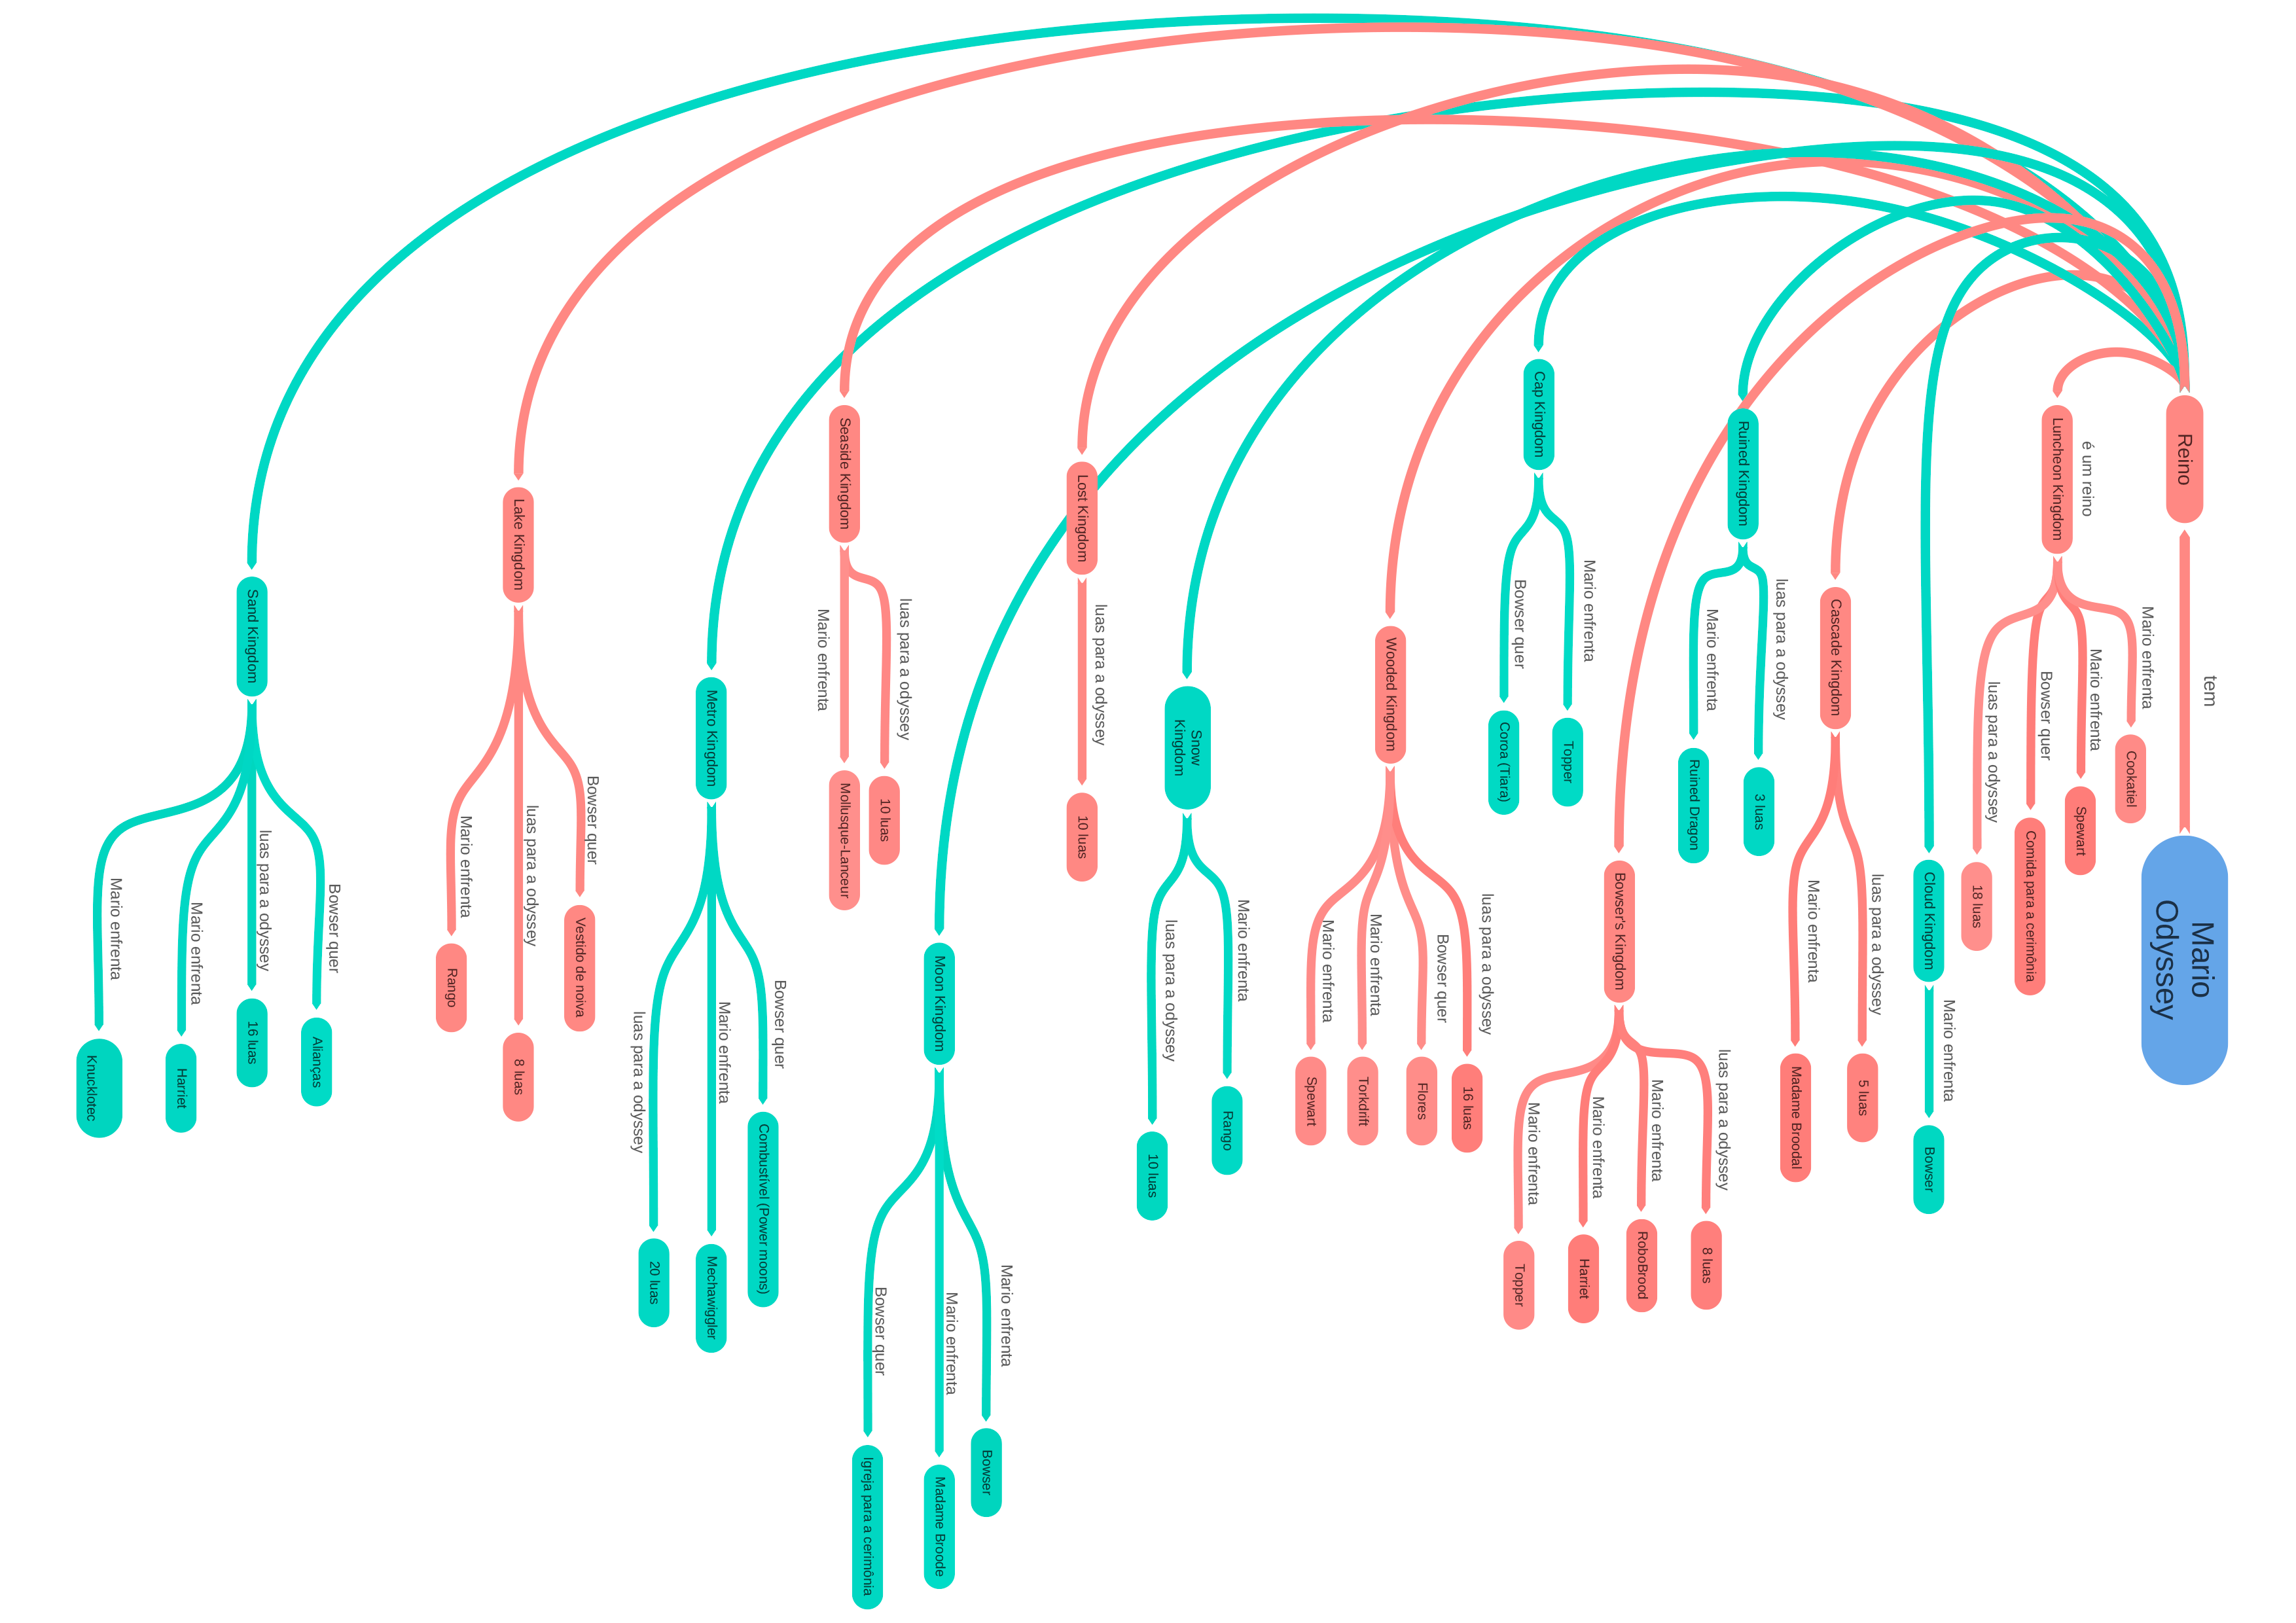
\includegraphics[width=23cm]{figuras/fig-diag-2} 
	\caption{Segunda parte do diagrama ontológico.}
	\label{fig-intro-diag2}
\end{sidewaysfigure}
\chapter{Dicionário de dados}
\label{sec-dicionario}

\section{Fatos}
	\begin{itemize}
		\item \textbf{personagem(nome):} define se o objeto dado é um personagem;
		\item \textbf{amigo(personagem):} define se o personagem é amigo de Mario;
		\item \textbf{inimigo(personagem):} define se o personagem é inimigo de Mario;
		\item \textbf{reino(entidade):} define se a entidade é um reino;
		\item \textbf{luas(reino, x):} indica a quantidade de luas necessárias para consertar a Odyssey naquele reino;
		\item \textbf{enfrentar(reino, inimigo):} indica o inimigo que Mario enfrenta em determinado reino;
		\item \textbf{deseja(reino, x):} indica o objetivo de Bowser naquele reino (se tiver);
		\item \textbf{vida\_base(X):} representa a quantidade de vida que o personagem inicia, assim como no jogo que se baseia, toda vez que obtemos uma lua, a vida do personagem é curado para sua vida base.		
	\end{itemize}

\section{Regras}
	\begin{itemize}
		\item \textbf{cls:} Função criada para limpar o terminal, funcionando apenas no Windows;
		\item \textbf{quant\_luas(R, L):} Determina a quantidade de luas em um reino dado, ou lista os reinos a partir de uma dada quantidade de luas;
		\item \textbf{quant\_casas(R, L):} Determina a quantidade de casas a partir de um reino, servindo para gerar as listas que corresponderão aos caminhos de cada reino;
		\item \textbf{qual\_adv(R, I):} Determina o boss a ser enfrentado em dado reino ou os reinos em que você enfrenta um dado boss;
		\item \textbf{criar\_lista(C,  L):} A partir de um número de casas, essa regra gera uma lista com o intervalo de 1 a C;
		\item \textbf{tem\_boss(R, B):} Determina se há ou não boss em um dado reino;
		\item \textbf{quant\_inim(L, B, QINI):} A partir de uma quantidade de luas, ele determina quantos inimigos devem haver em um reino para que você consiga escapar do reino;
		\item \textbf{posicionar\_inimigos(L, Q, C):} Gera uma lista de posições em que os inimigos devem ser posicionados em um reino, a partir da quantidade de casas e luas desse reino dado;
		\item \textbf{gerar\_lista(R, LU, C, L, LI, QI):} A partir de um reino dado, gera suas casas, quantidade de inimigos e os posiciona pelo reino, usando as regras anteriores;
		\item \textbf{casa\_vazia():} Dá para o usuário uma mensagem quando ele passar por uma casa em que não há inimigo marcado.
		\item \textbf{turno(H, HI, HF, HIF):} Recebe a vida dos personagens e realiza o turno do combate, atualizando as vidas após o turno;
		\item \textbf{atk\_turno(H, HF):} Realiza o ataque a um personagem com o HP dado, atualizando esse valor no segundo termo recebido pela regra.
		\item \textbf{batalha(H, HI, L):} Recebe a vida do personagem e adversário e a partir das funções anteriores, realiza os turnos do combate entre o personagem e o inimigo;
		\item \textbf{percorre(V, LI, C, B, HP, R):} Percorre o reino, analisando a lista de inimigos para saber em quais casas há inimigos e acionando a batalha onde houver;
		\item \textbf{carregar\_fase(R):} A partir de um reino dado, gera suas casas, inimigos, chefe e o percorre;
		\item \textbf{lista\_reinos(R):} Gera uma lista com o nome de todos os reinos a partir dos fatos;
		\item \textbf{mostrar\_reinos(R):} Mostra a lista de reinos gerada;
		\item \textbf{iniciar(A):} Mostra a lista de reinos e inicia o reino selecionado.
	\end{itemize}



	
	
\chapter{Análise}
\label{sec-analise}

Encontrei dificuldades em trabalhar com prolog que acontecem com qualquer outra nova linguagem de programação que nos lidamos: a sintaxe é diferente das outras linguagens e a forma de pensar em coisas que usamos constantemente em outras linguagens também, como o ato de percorrer listas, criar um loop, condições aninhadas e etc. Apesar das dificuldades, achei importante (e até um pouco divertido) repensar coisas que são meio que estabelecida em outras linguagens.


%%% Páginas finais do documento: bibliografia e anexos. %%%

% Finaliza a parte no bookmark do PDF para que se inicie o bookmark na raiz e adiciona espaço de parte no sumário.
\phantompart

% Marca o início dos elementos pós-textuais.
\postextual

% Referências bibliográficas
\bibliography{bibliografia}

% Índice remissivo.
\phantompart
\printindex

% Fim do documento.
\end{document}
